\documentclass[12pt
,headinclude
,headsepline
,bibtotocnumbered
]{scrartcl}
\usepackage[paper=a4paper,left=25mm,right=25mm,top=25mm,bottom=25mm]{geometry} 
\usepackage[utf8]{inputenc}
\usepackage[ngerman]{babel}
\usepackage{graphicx}
\usepackage{multirow}
\usepackage{pdfpages}
%\usepackage{wrapfig}
\usepackage{placeins}
\usepackage{float}
\usepackage{flafter}
\usepackage{mathtools}
\usepackage{hyperref}
\usepackage{epstopdf}
\usepackage[miktex]{gnuplottex}
\usepackage[T1]{fontenc}
\usepackage{mhchem}
\usepackage{fancyhdr}
%\setlength{\mathindent}{0pt}
\usepackage{amssymb}
\usepackage[list=true, font=large, labelfont=bf, 
labelformat=brace, position=top]{subcaption}
\setlength{\parindent}{0mm}

\setlength{\parindent}{0mm}

\pagestyle{fancy}
\fancyhf{}
\lhead{Ingenieurgeodäsie II\\Übung 12: Regression zur Höhenberechnung}
\rhead{Hsin-Feng Ho \\3378849}
\rfoot{Seite \thepage}
\begin{document}
	\section{a}
	Höhenanomalie
	\begin{align*}
		\zeta=h-H_N
	\end{align*}
wobei
\begin{itemize}
	\item $h$: ellipsoidische Höhe
	\item $H_N$: Normalhöhe
\end{itemize}
Höhenanomalien von Punkten 1-20:
\begin{table}[ht] \centering
	\begin{tabular}{|c|c|}
		\hline
		Pkt.Nr & Höhenanomalie [m] \\ \hline
		1     & 48,3548       \\ \hline
		2     & 48,3928       \\ \hline
		3     & 48,4118       \\ \hline
		4     & 48,4159       \\ \hline
		5     & 48,4290       \\ \hline
		6     & 48,3750       \\ \hline
		7     & 48,4098       \\ \hline
		8     & 48,4290       \\ \hline
		9     & 48,4360       \\ \hline
		10    & 48,4487       \\ \hline
	\end{tabular}
	\begin{tabular}{|c|c|}
		\hline
		Pkt.Nr & Höhenanomalie [m] \\ \hline
		11    & 48,3946       \\ \hline
		12    & 48,4203       \\ \hline
		13    & 48,4420      \\ \hline
		14    & 48,4556       \\ \hline
		15    & 48,4695      \\ \hline
		16    & 48,4148       \\ \hline
		17    & 48,4483       \\ \hline
		18    & 48,4659       \\ \hline
		19    & 48,4762       \\ \hline
		20    & 48,4890       \\ \hline
	\end{tabular}
\end{table}\\
Standardabweichung:
\begin{align*}
	\sigma_\zeta=\sqrt{\sigma^2_h+\sigma_{H_N}^2}=0,0051\,\mathrm{m}
\end{align*}
Graphische Darstellung:
\begin{figure}[h]
	\centering
	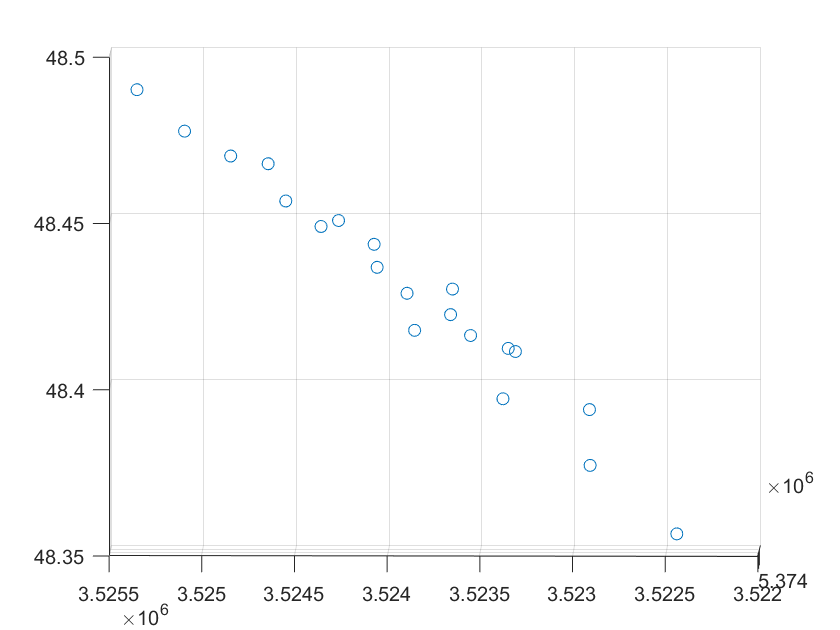
\includegraphics[width=12cm]{anomalie}
\end{figure}
\section{b}
In dieser Aufgabe sind die Höhenanomalien $\zeta_i$ mit einem Flächenpolynom von Grad 2 zu approximieren.
\begin{align*}
	\zeta_i=a_0+a_1y_i+a_2x_i+a_3y_ix_i+a_4y_i^2+a_5x_i^2                                           
\end{align*}
Mit Gauß-Markov-Modell stellt man die folgenden Gleichungen.
\begin{gather*}
	\underbrace{\begin{bmatrix}
			\zeta_1 \\
			\zeta_2 \\
			\vdots \\
			\zeta_{19} \\
			\zeta_{20}
	\end{bmatrix}}_{\text{$y$}} = \underbrace{\begin{bmatrix}
			1 & y_1' & x_1' & y_1' \cdot x_1' & y_1'^2 & x_1'^2 \\
			1 & y_2' & x_2' & y_2' \cdot x_2' & y_2'^2 & x_2'^2 \\
			\vdots \\
			1 & y_{19}' & x_{19}' & y_{19}' \cdot x_{19}' & y_{19}'^2 & x_{19}'^2 \\
			1 & y_{20}' & x_{20}' & y_{20}' \cdot x_{20}' & y_{20}'^2 & x_{20}'^2 \\
	\end{bmatrix}}_{\text{$A$}} \cdot \underbrace{\begin{bmatrix}
			a_0 \\
			a_1 \\
			a_2 \\
			a_3 \\
			a_4 \\
			a_5
	\end{bmatrix}}_{\text{$x$}} \\
	\hat{x} = (A^{T}A)^{-1}A^{T}y = \begin{bmatrix}
		48,4361 \\
		4,3398 \cdot 10^{-5} \\
		-2,5563 \cdot 10^{-6} \\
		8,1539 \cdot 10^{-9} \\
		-4,9588 \cdot 10^{-9} \\
		-5,7264 \cdot 10^{-9} \\
	\end{bmatrix}
\end{gather*}
Schwerpunktkoordinaten:
\begin{align*}
	x_s=\frac{1}{20}\sum_{i=1}^{20}x_i=5375436,408\,\mathrm{m}\quad
	y_s = \frac{1}{20} \sum_{i=1}^{20} y_i = 3523910,288\,\mathrm{m}
\end{align*}
\end{document}